比特币作为最经典的区块链项目,对其所采用的工作量证明的相关研究也最为丰富。迄今为止,比特币白皮书~\cite{nakamoto2008bitcoin}的引用次数已高达五千多次。本文选取共识层面几篇最据参考价值的文献进行调研。
\section{GHOST}
\subsection{介绍}
GHOST的全称是The Greedy Heaviest-Observed Sub-Tree,由Yonatan Sompolinsky和Aviv Zohar 在2015年提出\cite{sompolinsky2015secure}。其主要思想是对比特币最长链原则的一种修改。\footnote{比特币工作量证明可能会出现两个矿工几乎同时发现新的合法区块的情况,当他们同时公布自己新挖出得区块并接在当前主链上,这样就产生了分叉。比特币Nakamoto共识约定当前主链存在多个分叉时,将最长(即区块高度最高的)的分叉链最为唯一合法的链。}	

GHOST实现的主要目标是,在保证安全性的前提下给出了比特币的扩容方案。该共识思想已经成为以太坊升级项目的一部分。

\subsection{模型}
众所周知,比特币中存在$51\%$攻击,即需要假设作恶节点所占的算力比例不超过一半。这个假设在各大共识算法中都普遍存在。但GHOST认为,在比特币系统实际运作中,作恶节点实际需要占据的算力比例不需要$50\%$那么多即可发起攻击。


GHOST用$tree(t)$表示在时刻$t$整个区块链(所有区块)的结构。由于分叉的可能性,这个$tree(t)$不一定是一条链,而是“区块树”。

下面是GHOST模型的一些关键参数:
\begin{itemize}
	\item $\lambda_h$,表示诚实节点的出块速率,即新区快加入$tree(t)$的速率。值得一提的是,并不是所有的诚实节点出的区块都会最终出现在主链上,因为诚实节点之间也存在竞争,可能出现同时出块的情况进而产生分叉,
	\item $q\cdot\lambda_h,0<q<1$,表示作恶节点的出块速率。值得一提的是,作恶节点比诚实节点更团结——他(们)永远都只会在某一条秘密的链上进行挖矿,不会出现分叉。
	\item $s(T)$,$s$函数用于确定主链成员:输入一个子树$T$,输出一个区块,这个区块被确定为主链成员同时为下一个区块的父区块。比特币的最长链原则即让最长子链的起始区块作为$s$的返回值。
	\item $\beta$,表示主链增长的速度。注意只有$s$函数所决定的区块才能被主链记录。
	\item $TPS=\beta(\lambda,b)\cdot K$,其中$b$为区块大小(KB),K为平均每KB数据包含的交易数目。
\end{itemize}
在比特币最长链原则下,针对传统的$51\%$攻击,GHOST认为,\textbf{需要竞争的是(诚实节点带来的)主链增长速度与作恶节点的秘密链的增长速度,即$\beta$与$q\cdot\lambda_h$,而不简单的是用出块速率$\lambda_h$来对比。}所以,GHOST把$\frac{\beta}{\lambda_h}$作为所谓的“安全系数”,即当且仅当$q>\frac{\beta}{\lambda_h}$时作恶节点将会成功攻击(传统认为需要$q>1$才能进行攻击)。
	
\subsubsection{对比特币扩容的思考}
比特币的低TPS一直是人们诟病的原因。两种简单的提升TPS的想法为:
\begin{itemize}
	\item 增加每个区块的大小。(增大$b$,比特币的区块平均大小为1MB)
	\item 减小区块出块的平均间隔时间。(增加$\lambda_h$,目前比特币的平均间隔为10分钟)
\end{itemize}
根据定义,咋看之下这两种方式确实能提升TPS,但\textbf{GHOST指出这两中简单的方法都存在一系列问题。而这也是GHOST这篇论文的主要贡献。}

1.增加区块大小$b$

随着区块容量的变大,当矿工挖到新的区块时需要更长的时间来广播,同时用户也要花更长的时间来同步实时的区块链状态。这意味着新的区块需要花更长的时间被主链接收且被绝大多数节点验证,这样会导致更容易产生孤块,更容易发生分叉,安全性降低,主链增长速度反而会受到影响。有调研表明在维持基本的安全性的情况下比特币区块容量不能超过8M。

2.增加出块速率$\lambda_h$

注意到当$\lambda_h$增加时,直接影响是安全系数$\frac{\beta}{\lambda_h}$降低了。原因是诚实节点和作恶节点的出块速率都会增加,同时也会造成状态同步压力变大,分叉变多,主链增长速率$\beta$的提升受限。

所以,GHOST对简单的通过增加区块大小和降低出块时间的比特币扩容进行了否定。

\subsection{GHOST算法}
如前所述,GHOST的核心思想是将比特币的最长链原则改为最重子树原则。

对一个区块$B$,定义$subtree(B)$为以$B$为根的子树,$Children(B)$为$B$的直接子区块。写下来我们将实现GHOST中的$s$函数,用于决定一棵树被选为主链的块。

\begin{algorithm}[H]
	\caption{GHOST}%算法名字
	\KwIn{Block Tree $T$}
   set $B \leftarrow Genesis Block$\;
	\eIf {$Children(B)=\emptyset$}
    {Return $B$ and exit\;}
   {Update $B\rightarrow \arg\max_{C \in Children(B)}|subtree(C)|$\;}
	GOTO line 2\;
\end{algorithm}
其核心思想如\reffig{fig:GHOST1}(1B,2C,3D这几个区块相比其兄弟区块拥有更重的子树。)
\begin{figure}
	\centering
	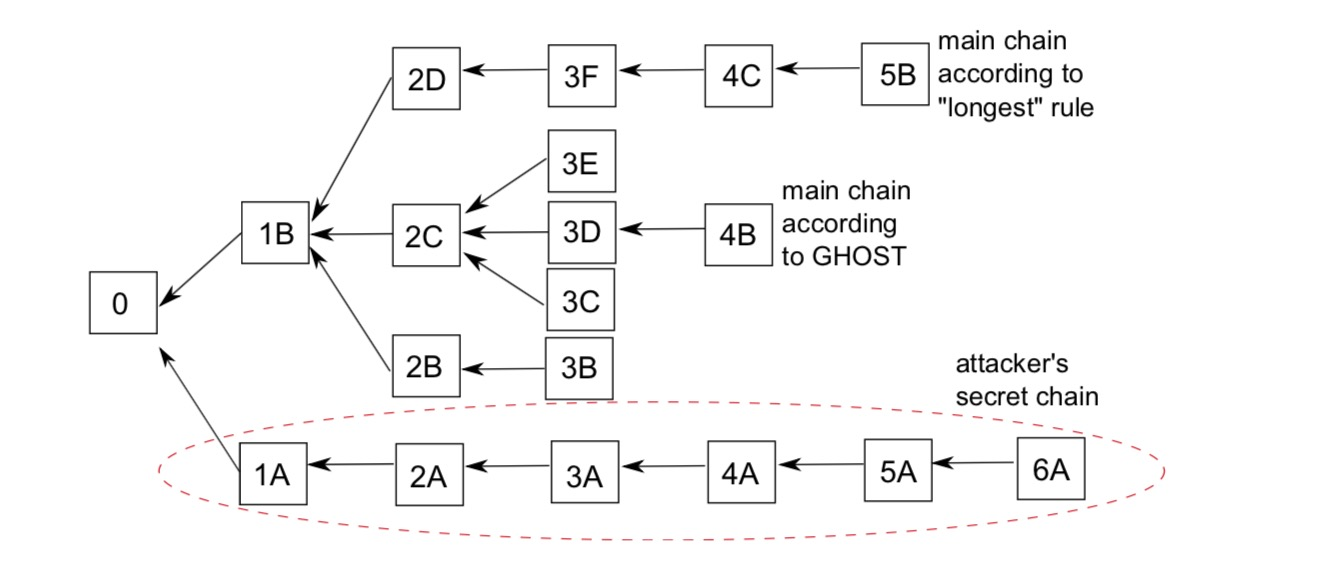
\includegraphics[width=1\textwidth]{../common/GHOST_1.png}
	\caption{GHOST中的最重子树} 
	\label{fig:GHOST1}
\end{figure}


\subsection{性质分析}
相比于比特币的最长链原则,GHOST的主要性质是安全系数能独立于区块产生的速度,始终为1(即能抵抗$50\%$的攻击)。这个性质由下面两个引理保证:
\begin{lemma}
	定义$\psi_B$为区块$B$或者被所有节点接受,或者被所有节点所拒绝的时刻。那么$Pr(\Psi_B<\infty)=1$且$E[\Psi_B]<\infty$
\end{lemma}
即这个引理保证最终一致性。和比特币一样,GHOST不存在finality状态,故这个一致性也是概率上的。这个引理的证明思想是,出现不一致性仅当存在两个重量相同的子树。那么存在一个时刻,在一段时间内只挖出一个区块且在之后进行广播的过程中也没有新的区块被挖出,那么平衡将被打破,最重子树得以确定。

GHOST的抵抗$50\%$以下攻击由下面的引理决定:
\begin{lemma}
	如果$0<q<1$,假设区块$B$已经在主链上出现的时间趋于无穷大,那么它被排出主链的概率趋近于0。
\end{lemma}
由于这个结论与$\lambda_h$无关,这就为GHOST的扩容提供了保证。下面两张图给出了GHOST的TPS及安全系数随$\lambda_h$的变化。

\begin{figure}
	\centering
	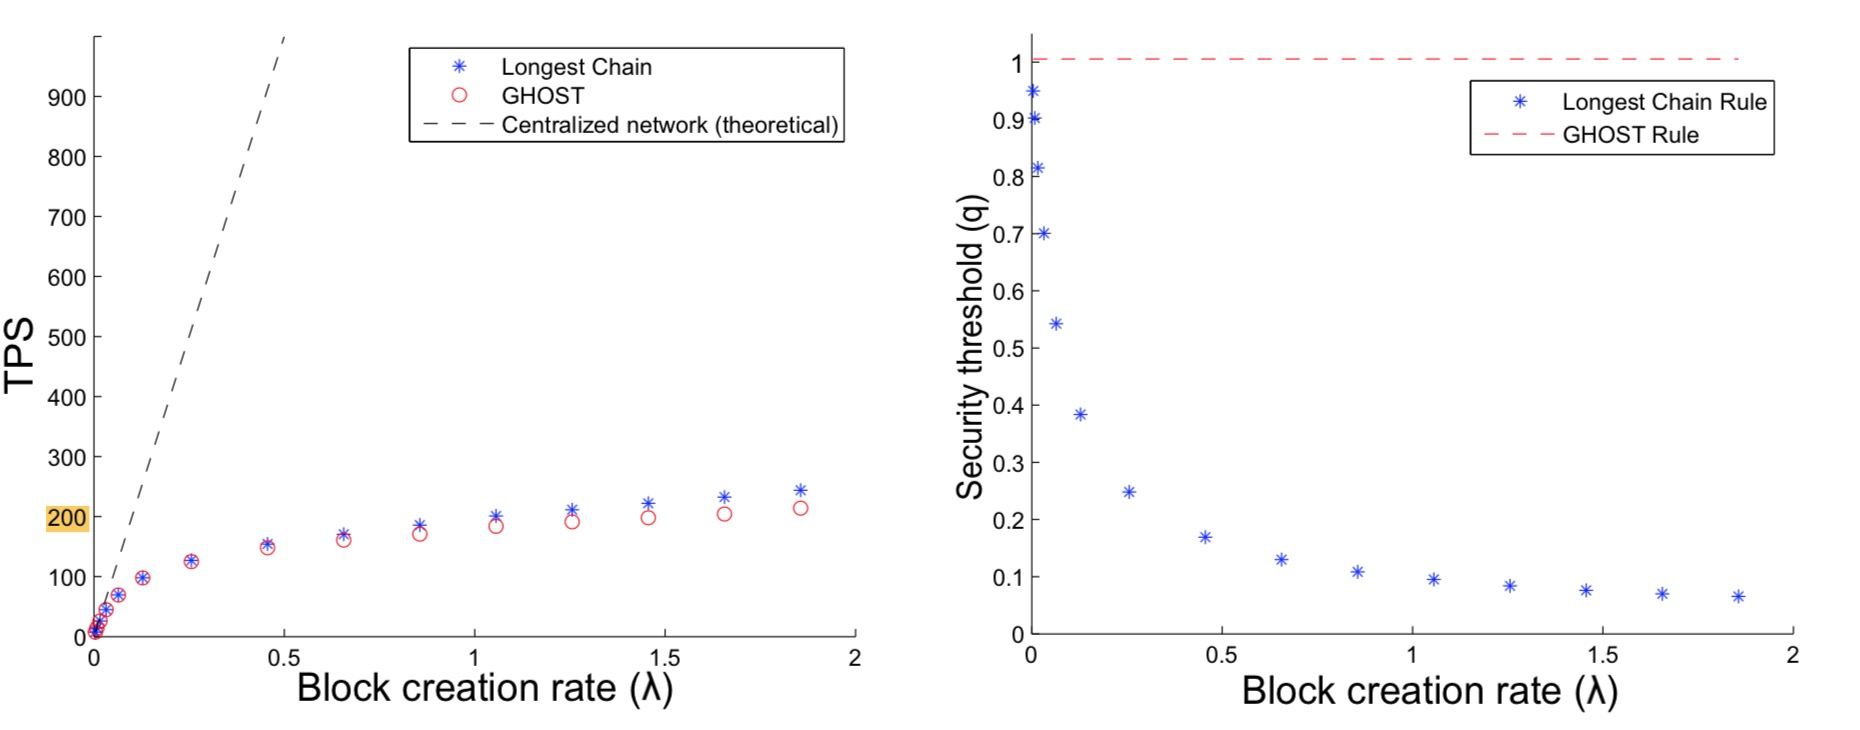
\includegraphics[width=1\textwidth]{../common/GHOST_2.png}
	\caption{TPS与安全系数的变化} 
	\label{fig:GHOST2}
\end{figure}

所以,当$\lambda_h$达到一定数值后TPS可以达到200左右,若再继续增大整个系统的同步会受影响,安全性降低,故对主链增长及TPS的提升很小。

文章最后还有一些关于主链增长速度的定理。这里不做详细介绍。
\subsection{总结}
GHOST给我们最大的其实是不能简单地靠增加出块速率和区块大小来增加TPS。设计共识算法是可以不局限于最长链原则。


	

